\section{Resultados y discusiones}

Los resultados se presentan a continuación en el orden en el que se emplean 
los pasos en la librería \path{galpynostatic} de Python: una primera sección
para el preprocesamiento de los datos experimentales, luego otra para el ajuste
de estos datos con el modelo heurístico, y, por último, la utilización de éste
para predecir las condiciones del tamaño de partícula para lograr una carga
rápida de 15 y 5 minutos. Sumado a esto, también se compara el comportamiento que
tendrían los distintos materiales, dados sus parámetros fundamentales, a 
distintos tamaños.

\subsection{Preprocesamiento de los datos experimentales}

Un procedimiento experimental usual para evaluar los materiales de las baterías
consiste en medir los perfiles galvanostáticos a distintos valores de C-rate.
En la Figura \ref{fig:preproc} se muestran como ejemplo las mediciones realizadas
por Wang \textit{et al.} \cite{wang2019high} para LiCoO$_2$ (LCO) recubierto con 
TiO$_2$. Además, se agrega una línea punteada horizontal que se corresponde
con el potencial de equilibrio reportado en el trabajo citado, 3.9 V, y otra
0.15 V por debajo, que es el valor que corresponde al potencial de corte
elegido en este capítulo. Esta es la región de interés en el gráfico, ya que 
los valores en los que el SOC se intersecta con esta última curva (SOC$_{\max}$)
son los que se utilizan para ajustar el modelo en función de C-rate.
\begin{figure}[h!]
    \centering
    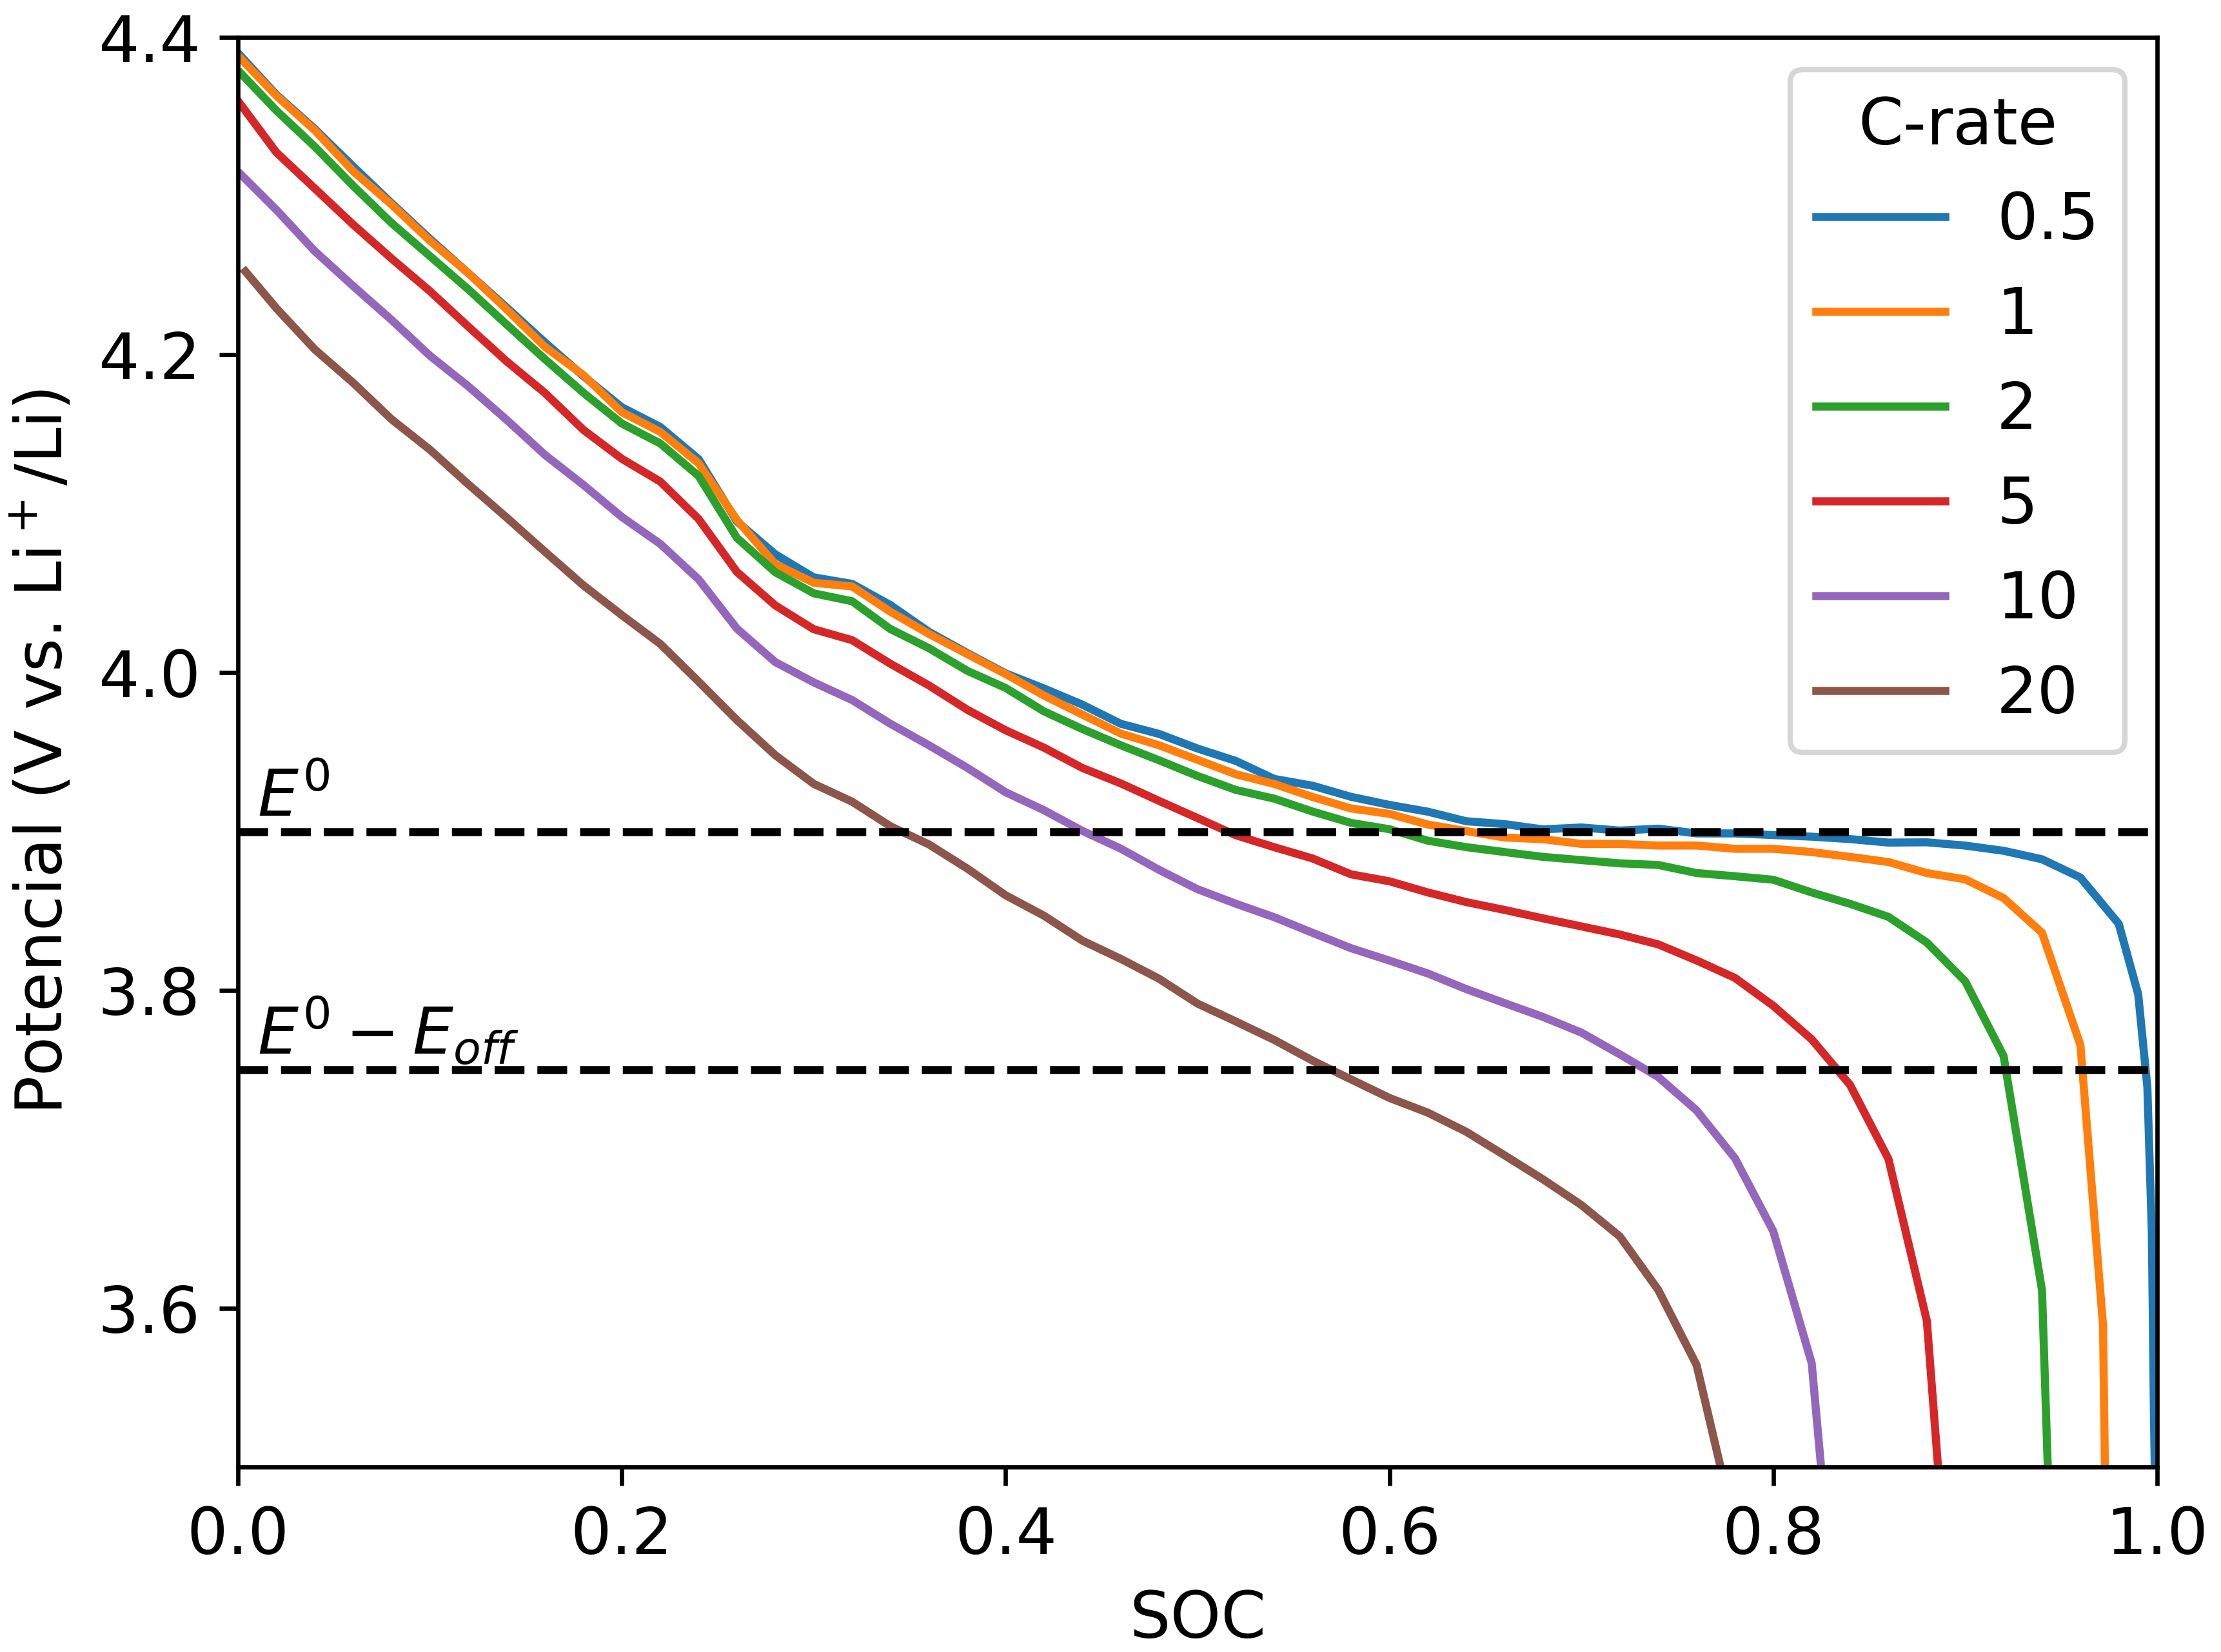
\includegraphics[width=0.7\textwidth]{FastCharging/un/resultados/preprocesamiento/preprocesamiento.png}
    \caption{Perfiles galvanostáticos para distintos valores de C-rate para el
    sistema LCO recubierto de TiO$_2$. Las líneas horizontales indican el 
    potencial de equilibrio y el de corte utilizado para determinar la 
    capacidad máxima normalizada alcanzada (SOC$_{\max}$) a cada C-rate. 
    Reproducido del trabajo de Wang \textit{et al.} \cite{wang2019high}.}
    \label{fig:preproc}
\end{figure}

Es importante destacar que, en el trabajo citado, los perfiles galvanostáticos
se presentan en función del SOC normalizado, que no siempre es el caso. La 
forma usual en la que estos resultados son reportados es en función de la 
capacidad de descarga. En estos casos, es necesario normalizarla con respecto
a la capacidad máxima ($Q_{\max}$) alcanzada por el material, para así obtener
el SOC normalizado. El criterio utilizado en este capítulo para encontrar 
$Q_{\max}$ fue considerar el valor máximo de la capacidad alcanzado por la 
medición a la C-rate más baja. Gráficos similares al presentado en la Figura 
\ref{fig:preproc} son obtenidos en el resto de los trabajos experimentales que
se utilizan en los ajustes que siguen.


% Copyright (c) 2024, Francisco Fernandez
% License: CC BY-SA 4.0
%   https://github.com/fernandezfran/thesis/blob/main/LICENSE
\subsection{Ajuste de dos conjuntos de parámetros DFTB}

Como fue introducido en la sección \ref{s:dftb}, para el método DFTB hay dos 
grupos de parámetros a ser determinados, los electrónicos (los orbitales 
pseudoatómicos y las densidades electrónicas) y los potenciales repulsivos para 
cada par de elementos químicos (Si-Si, Si-Li y Li-Li). La optimización de cada 
uno de ellos está sujeta a reproducir alguna propiedad deseada, como la 
estructura de bandas, las energías de atomización, entre otras. Para el ajuste
de la estructura de bandas se siguió el trabajo de van den Bossche \cite{van2019},
considerándose para el Li los electrones de valencia 2s mientras que para el Si 
los 3s y los 3p. La comparación de la estructura de bandas entre DFTB y DFT para 
los conjuntos A y B de parámetros se analiza en profundidad en la referencia 
\cite{oviedo2023}.

Para la parametrización del potencial de repulsión de cada uno de los conjuntos 
A y B se siguió el algoritmo de ajuste descripto en la sección \ref{s:algfit}
que permite optimizar los pesos de cada una de las estructuras en el conjunto de 
entrenamiento. Los coeficientes $\check{\boldsymbol{\xi}}_s$ minimizados para cada
conjunto, A y B, se reportan en la Tabla \ref{t:xiweights}.
\begin{table}[b]
    \centering
    \caption{Pesos óptimos, $\check{\boldsymbol{\xi}}_s$, de cada conjunto.}
    \setlength\extrarowheight{2pt}\stackon{%
    \begin{tabular}{l c c}
        \toprule
        \textbf{$s$} & 
        \textbf{conjunto A} & 
        \textbf{conjunto B} \\ 
        \midrule
        Li & $0.23\times10^{-2}$ & 0.49 \\
        Li$_{15}$Si$_4$ & 0.15 & 0.28$\times10^{-21}$ \\
        Li$_{13}$Si$_4$ & 0.21 & 0.17$\times10^{-1}$ \\
        Li$_7$Si$_3$ & 0.21 & 0.11$\times10^{-1}$ \\
        Li$_{12}$Si$_7$ & 0.23 & 0.11$\times10^{-2}$ \\
        LiSi & 0.21 & 0.35$\times10^{-3}$ \\
        Si & 0.83$\times10^{-7}$ & 0.49 \\
        \bottomrule
    \end{tabular}
    }{}
    \label{t:xiweights}
\end{table}
Es interesante que para el conjunto A el algoritmo reduce los pesos relativos del 
Li y del Si puro y aumenta los de las aleaciones. Mientras que para el conjunto 
B sucede lo contrario, los pesos óptimos son mayores para los elementos puros y
menores para las aleaciones. Este comportamiento se debe a que el término de la 
energía de bandas del conjunto A se construye utilizando los elementos puros 
mientras que el mismo término para el conjunto B utiliza una de las aleaciones. 
Resulta razonable que el término de repulsión, que busca compensar el residuo de la 
energía dada por todas las demás contribuciones energéticas, sea menos importante 
para las estructuras consideradas en el ajuste de las energías de banda y más 
importante para el resto. Así, los coeficientes óptimos $\check{\boldsymbol{\xi}}_s$ 
parecen ser capaces de percibir esta situación y tratar de compensarla al centrar 
la parametrización en las estructuras que más la necesitan.

Otra observación que surge de la Tabla \ref{t:xiweights} es el peso relativo bajo
que resulta en ambos conjuntos para la aleación cristalina Li$_{15}$Si$_4$, en 
comparación con el resto de las aleaciones. En particular, para el conjunto B este 
peso es prácticamente igual a cero, indicando que la inclusión de estas 
estructuras en el conjunto de entrenamiento no contribuye a una mejora de la 
predicción de las energías de formación relativas. Esto puede deberse a que la 
estructura de Li$_{15}$Si$_4$ tiene una naturaleza particular que difiere del 
resto de las aleaciones e interfiere de alguna manera con el ajuste de los 
parámetros del modelo. Por ejemplo, una explicación posible puede ser que el 
entorno químico de esta estructura es bastante diferente al del resto de las 
aleaciones por lo que la predicción global puede ser mejorada al centrar el 
ajuste en el resto de las aleaciones. En este sentido, el procedimiento de 
optimización propuesto en este capítulo puede considerarse como una herramienta 
para detectar peculiaridades dentro del conjunto de entrenamiento.


\subsection{Predicción del tamaño óptimo de partícula}

Como ya ha sido mencionado a lo largo de esta tesis, el criterio de carga rápida
está definido por la obtención del 80\% de la capacidad del electrodo en 15 
minutos, lo cual se traduce en un SOC$_{\max}$ de 0.8 y una C-rate de 4 C. La
Figura \ref{fig:prediccion} muestra donde se encuentra cada sistema analizado en
el diagrama $\log(\Xi)$--$\log(\ell)$ para dicha C-rate. También se presenta una
curva de nivel con una línea roja correspondiente a SOC$_{\max} = 0.8$. Puede
observarse que tres de los materiales ya se encuentran en la región de 
SOC$_{\max}$ mayor a 0.8 (LCO, LMNO y LNMO), mientras que los otros se encuentran
por debajo de este valor (LTO, Grafito amorfo y LFP).
\begin{figure}[h!]
    \centering
    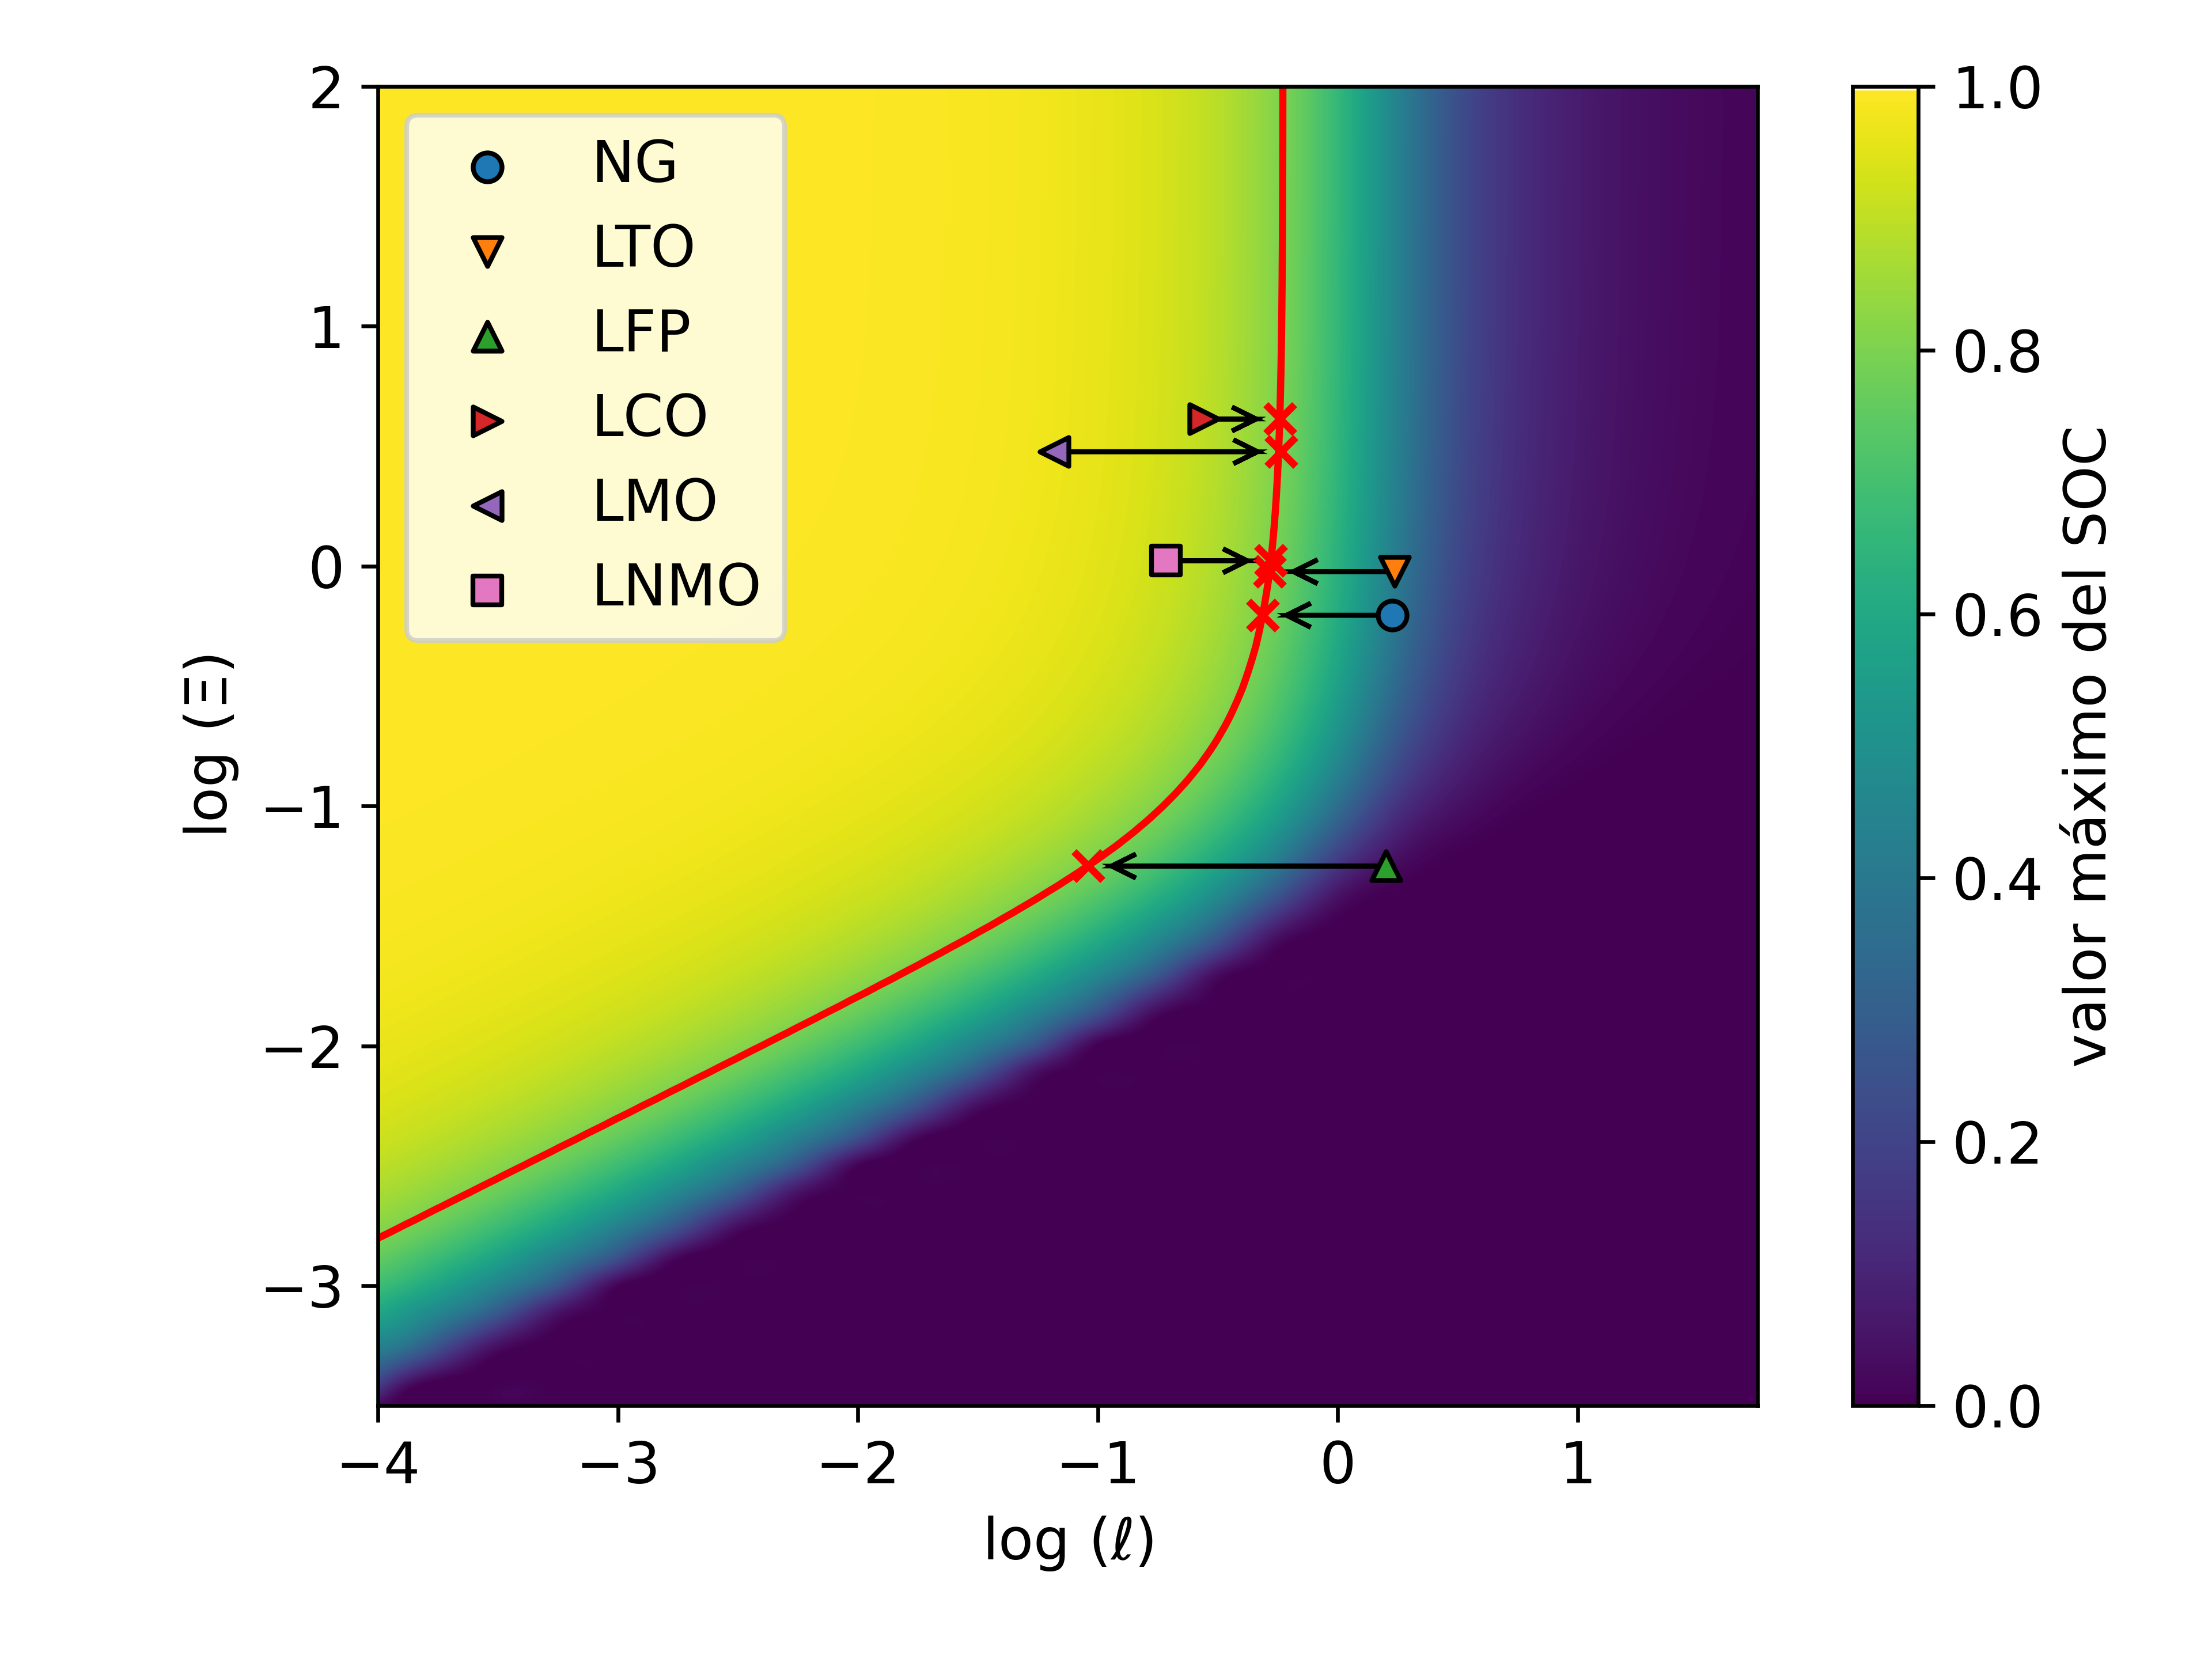
\includegraphics[width=0.7\textwidth]{FastCharging/un/resultados/prediccion/prediccion.png}
    \caption{Diagrama de SOC$_{\max}$ mostrando la ubicación de los materiales 
    usuales de LIBs a 4 C para las referencias consideradas \cite{mancini2022,
    he2012, lei2015, wang2019high, bak2011, nishikawa2017}. En los casos en los 
    que la curva de cargado a 4 C no estaba disponible, el valor del punto fue 
    predicho con el modelo. La línea roja muestra la curva de nivel 
    correspondiente al valor 0.8 de SOC$_{\max}$. Las flechas muestran el cambio
    en el tamaño de la partícula que debería efectuarse para obtener dicho valor
    a la C-rate dada. Las curces sobre la línea muestran la posición de estos
    tamaños de partícula nuevos.}
    \label{fig:prediccion}
\end{figure}
Haciendo uso del diagrama se puede predecir una forma simple y rápida el tamaño 
de partícula requerido para satisfacer el criterio de carga rápida. Dado que los
valores de $D$ y $k^0$ ya fueron ajustados, el valor de $d$ seleccionado por el
experimento y el de C-rate por el criterio, el valor de $\Xi$ es constante. Luego,
para alcanzar el valor de 0.8 de SOC$_{\max}$ hay que variar $\ell$ y esto se
logra disminuyendo o aumentando el tamaño de la partícula, según sea necesario. 
Este desplazamiento necesario está representado por las flechas en la Figura 
\ref{fig:prediccion} para cada caso. Ya se ha apreciado que tres sistemas se 
encuentran en la región ya optimizada (LCO, LMO y LNMO), por lo que en estos casos
los tamaños predichos para alcanzar SOC$_{\max} = 0.8$ a 4 C serán mayores que 
los experimentales. Por el contrario, el resto de los materiales (LTO, Grafito
amorfo y LFP) tienen que ser mejorados con una reducción del tamaño de partícula
para cumplir la condición. En la tabla \ref{t:prediccion} se muestran los tamaños
de partícula predichos para todos los materiales en la tercera columna para este
criterio. Las incertidumbres se determinaron por propagación de errores con 
derivadas parciales. Ya que el tamaño de la partícula sólo aparece en el parámetro
$\ell$, al definir $\ell_{\text{opt}}$ como el valor al cual el SOC$_{\max}$ 
alcanza el valor deseado de 0.8 y usar que $V/A = d/z$ se puede despejar de la 
ecuación \ref{eq:ele} que
\begin{equation}
    d = \sqrt{\frac{t_h z D 10^{\ell_{\text{opt}}}}{C_r}}.
\end{equation}
Si además se supone que toda la incertidumbre está asociada al coeficiente de 
difusión $D$, al cual ya se le calculó su incerteza, se puede obtener que
\begin{equation}
    \Delta d = \frac{1}{2} \sqrt{\frac{t_h z 10^{\ell_{\text{opt}}}}{C_r D}} \Delta D.
\end{equation}

\begin{table}[h!]
    \centering
    \caption{Tamaño experimental y valores predichos para cargar el 80\% del
    electrodo en 15 y 5 minutos.} 
    \setlength\extrarowheight{2pt}\stackon{%
    \begin{tabular}{l c c c}
        \toprule
        \textbf{Material del} &
        \textbf{Tamaño} &  
        \textbf{Tamaño predicho} & 
        \textbf{Tamaño predicho} \\
        \textbf{electrodo} & 
        \textbf{experimental [$\mu$m]} &  
        \textbf{para 15 minutos [$\mu$m]} & 
        \textbf{para 5 minutos [$\mu$m]} \\
        \midrule
        Grafito amorfo & 7.5 & 4.027 $\pm$ 0.002 & 2.167 $\pm$ 0.001 \\
        LTO & 1.75 & 0.962 $\pm$ 0.004 & 0.530 $\pm$ 0.002 \\
        LFP & 0.35 & 0.084 $\pm$ 0.002 & 0.0309 $\pm$ 0.0006 \\
        LCO & 20 & 28.8 $\pm$ 0.6 & 16.4 $\pm$ 0.4 \\
        LMO & 0.025 & 0.0734 $\pm$ 0.0003 & 0.0418 $\pm$ 0.0002 \\
        LNMO & 7.999 & 13 $\pm$ 2 & 7.3 $\pm$ 0.8 \\
        \bottomrule
    \end{tabular}
    }{}
    \label{t:prediccion}
\end{table}

Al observarse un buen desempeño para la carga de 15 minutos, se puede exigir un 
poco más que este criterio y predecir el tamaño de partícula requerido para una
C-rate más alta, digamos 80\% de la carga en 5 minutos (12 C). Si bien esta figura
puede parecer sobredemandante a primera vista, reportes recientes consideran 
protocolos de carga de 10 minutos \cite{mattis2021, attia2020}. Los resultados
se muestran en la última columna de la Tabla \ref{t:prediccion}. Como puede 
observarse, el comportamiento depende del sistema y del experimento en particular
considerado. El único caso donde se cumple este último criterio de carga rápida 
es el LMO, ya que el tamaño experimental sobrecumple el criterio. Aunque el LCO 
y el LNMO no cumplen con este último criterio, los cambios en sus tamaños serían
menores, por lo que estos materiales requieren mejoras menores. En el resto de 
los casos, para el LFP se necesitaría una disminución de un orden de magnitud 
en su tamaño, mientras que para el grafito amorfo o el LTO se requeriría una
disminución de su tamaño en un factor de 3.


\subsection{Comparación de sistemas con un mismo tamaño}

La curva de los distintos experimentos ajustados sigue el mismo comportamiento 
para todos los sistemas, como se mostró en la Figura \ref{fig:ajustes-mapa},
esto es un efecto esperado debido a las definiciones de $\Xi$ y $\ell$, todas las
curvas exhiben una pendiente de $-1/2$ dada por la siguiente ecuación
\begin{equation}
    \log(\Xi) = \log(B) - \frac{1}{2}\log(\ell),
\end{equation}
donde el valor de $B$ puede obtenerse al eliminar C-rate de las ecuaciones 
\ref{eq:xi} y \ref{eq:ele} para obtener
\begin{equation}
    \log(\Xi) = \log\left(\frac{k^0 d}{D \sqrt{z}}\right) - \frac{1}{2}\log(\ell),
\end{equation}
donde se ve que la ordenada al origen contiene una composición de los parámetros
fundamentales considerados. 

\begin{figure}[t]
    \centering
    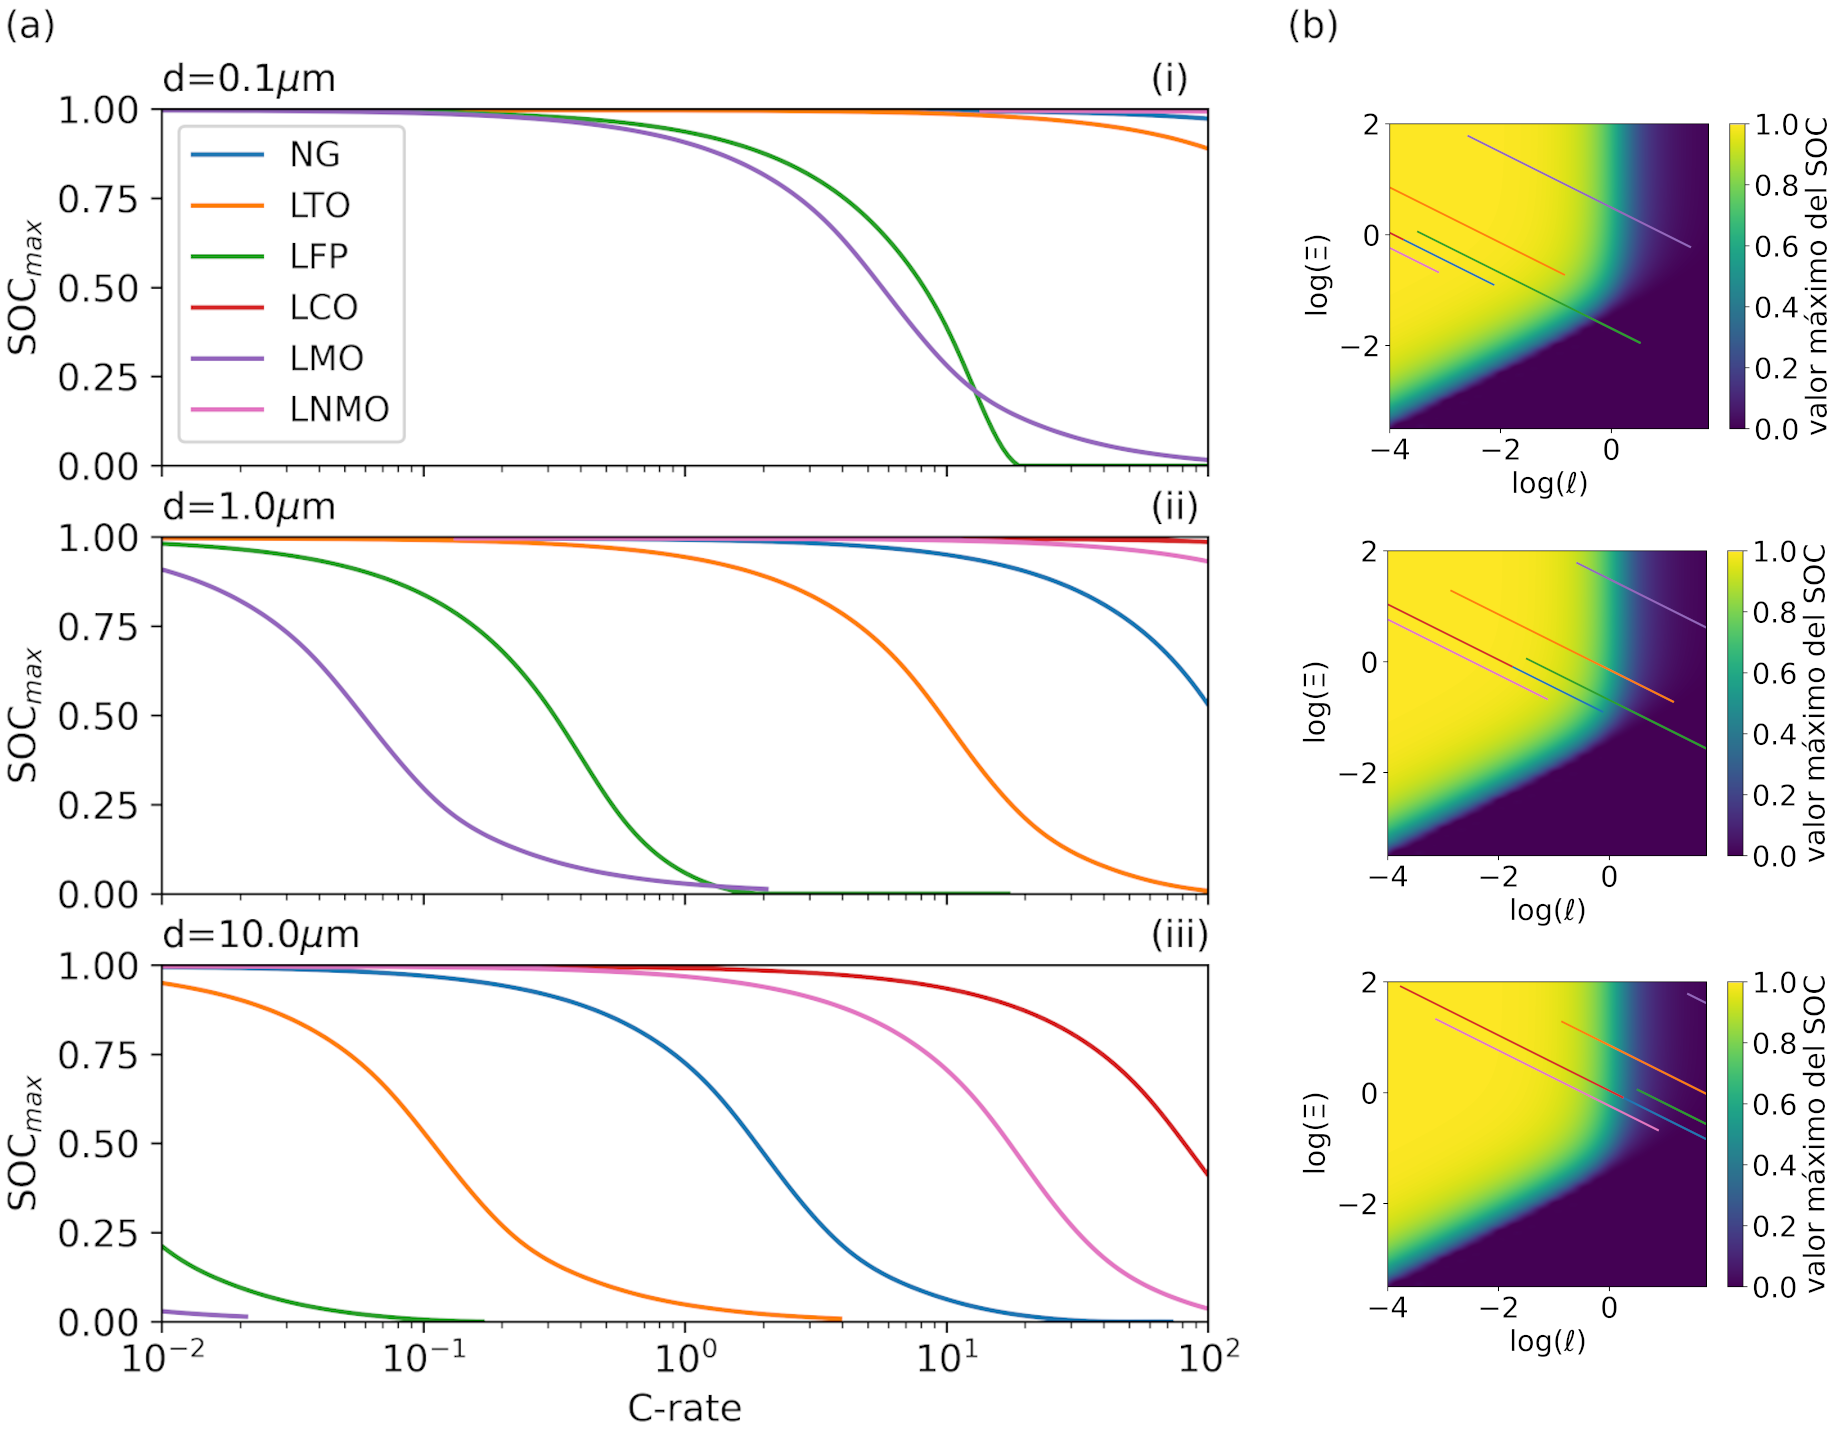
\includegraphics[width=\textwidth]{FastCharging/un/resultados/comparacion/comparacion.png}
    \caption{Comparación de los sistemas considerados con distintos tamaños de 
    partícula entre 0.1 $\mu$m y 10.0 $\mu$m en el rango experimental usual para 
    valores de C-rates: (a) SOC$_{\max}$ \textit{versus} C-rate. (b) Diagramas.}
    \label{fig:comparacion}
\end{figure}

Si se quieren comparar los méritos de los distintos materiales, en términos de 
sus propiedades intrínsecas de transferencia de carga en la interfase 
electrodo/electrolito ($k^0$) y difusión de iones dentro de ellos ($D$), se 
debería comparar el comportamiento de las partículas para un mismo tamaño a 
distintas C-rate, lo cual se presenta en la Figura \ref{fig:comparacion}. En 
particular, en la Figura \ref{fig:comparacion}a se muestra el SOC$_{\max}$ 
en función de la C-rate, considerando un conjunto de tamaños de partículas y 
C-rates en un rango físicamente razonable. Para obtener estos resultados se 
utilizaron los valores de $D$ y $k^0$ ajustados en la sección \ref{s:ajustes}.

En el gráfico (i) de la Figura \ref{fig:comparacion}a para 0.1 $\mu$m está
claro que los únicos materiales que muestran una pérdida de la capacidad para
C-rates altas son LFP y LMO, el resto retiene más del 80\% de la capacidad, 
incluso a 100 C. En el segundo gráfico (ii) de la Figura
\ref{fig:comparacion}a para 1 $\mu$m, el LTO y el NG tienen
una caída en el SOC por debajo del 50\% para 100 C, mientras que LCO y LNMO
están por encima del 80\%. Por último, el tamaño de partícula más grande que se 
considera, 10 $\mu$m (Figura \ref{fig:comparacion}a, gráfico (iii)), 
todos los materiales presentan una retención de la capacidad por debajo del 80\%
a la C-rate más alta. En la Figure \ref{fig:comparacion}b estos datos 
comportamientos están presentados en el diagrama construido con las simulaciones
galvanostáticas para dar una idea de las regiones en las que cada sistema se
encuentra. 

Cabe destacar que la secuencia de materiales dada en la Figura 
\ref{fig:comparacion} fue obtenida utilizando los valores de $k^0$ y $D$ 
ajustados con el modelo a los datos experimentales. Ajustar otros experimentos
podría alterar esta secuencia. Idealmente, las mediciones deberían estar 
realizadas sobre electrodos de una sola partícula.

